%%%%% RESULTS %%%%%%
t\section{Results}
\label{sec:results}

Figure \ref{fig:fidelity_plot} displays the haptic feedback fidelity and versatility scores of the systems described in each article. The quality score of each system is depicted by the dot's color and size, respectively (see section \ref{sec:quality}).


\subsection{Search Results}

%%%% Rewrite for precise numbers!! %%%%%

The search yielded 404 results, which were saved in the library of Mendeley. 75 duplicates were found and removed. The remaining 329 records were screened based on title and abstract first. This led to the preliminary exclusion of 290 records, of which 73 records were re-screened as they were from the years 2022-2024 (see fig. \ref{fig:prisma}), along with 3 papers that had been included based on citation search. 
65 records were excluded during this screening.

In total, 50 articles were eligible for the full-text screening. Of these, 14 were excluded based on the exclusion criteria, and the remaining 36 studies were included in this review.


\subsubsection{Study characteristics}
\paragraph{Year of publication}
The included studies' publication dates from 2000 to 2024. As seen in \ref{fig:years}, the number of studies has greatly increased in the past decade, with a peak in 2018.

\begin{figure}[htbp]
    \centering
    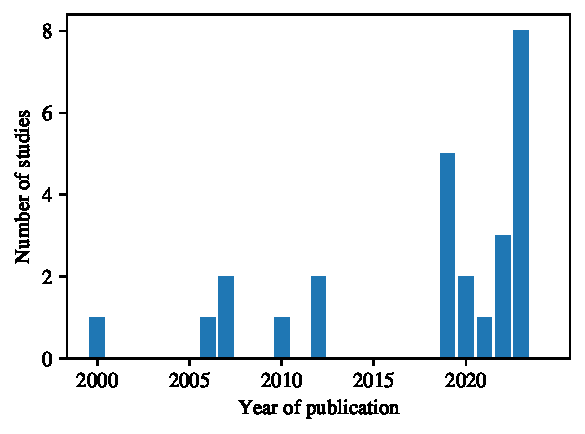
\includegraphics[width=\columnwidth]{figures/years.pdf} 
    \caption{Publication dates of the included articles}
    \label{fig:years}
\end{figure} 


\paragraph{Body parts involved}
% Graph to quantify involved body parts (pie chart)

Figure \ref{fig:body_parts_pie} shows which body parts were involved in the studies. As can be seen, most studies were concerned with stimuli at the palm and fingers, and many experiments also involved the forearm and upper arm. The fewest studies involved the feet, namely, the experiments with the DaVinci Research Kit \cite{Caccianiga2021, Oquendo2024}.

\begin{figure}[htbp]
    \centering
    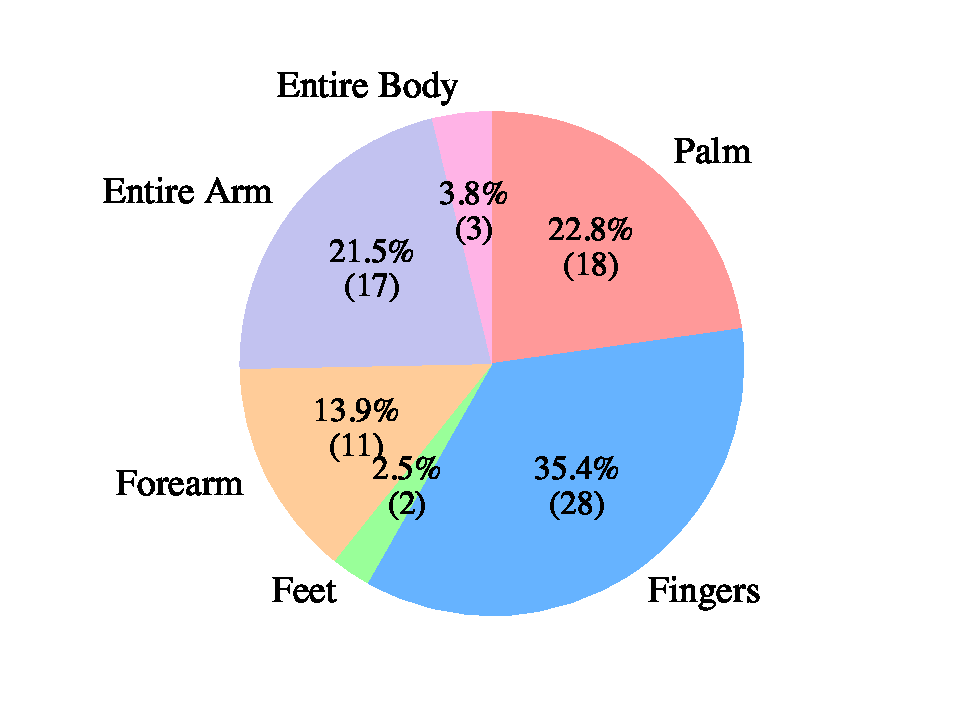
\includegraphics[width=\columnwidth]{figures/body_pie.pdf} 
    \caption{Body parts involved in the studies}
    \label{fig:body_parts_pie}
\end{figure} 

\subsection{Search Analysis Results}

\subsubsection{Clustering of the data}
The papers were evaluated based on the haptic fidelity framework by Muender et al. \cite{Muender2022HapticReality} and plotted based on their haptic fidelity and versatility score as can be seen in figure \ref{fig:fidelity_plot}. The plot also shows the different confidence scores based on the quality of the papers. 

\begin{figure*}[htbp]
\begin{tikzpicture}[scale=3.9]
    
    % Add axis labels
    \foreach \x in {0,0.5,1,1.5,2} {
        \draw [very thin, lightgray](\x*2 cm, 0-0.05) -- (\x*2 cm, 2+0.05) node[anchor=north] {};
        \draw [very thin, lightgray](0-0.05,\x cm) -- (4+0.05,\x cm) node[anchor=east] {};
    }

    % Draw the horizontal & vertical dotted lines
    \draw[dashed, thick, dottedlines] (4/3,0) -- (4/3,2);
    \draw[dashed, thick, dottedlines] (8/3,0) -- (8/3,2);
    \draw[dashed, thick, dottedlines] (0,2/3) -- (4,2/3);
    \draw[dashed, thick, dottedlines] (0,4/3) -- (4,4/3);

    % Draw axes
    \draw[thick,<->] (0,1) -- (4,1) node[anchor=south west] {\parbox{2cm}{Haptic \\ Fidelity}};
    \draw[thick,<->] (2,0) -- (2,2) node[anchor=south] {Versatility};

    \node at (0,0.92) {\scriptsize{abstract}};
    \node at (2.3,0.92) {\scriptsize{representational}};
    \node at (4,0.92) {\scriptsize{realistic}};
    \node at (1.8,0.05) {\scriptsize{specific}};
    \node at (1.8,1.07) {\scriptsize{broad}};
    \node at (1.8,1.95) {\scriptsize{generic}};

    % Legend
    \draw[fill=white] (0.08,1.9) rectangle (1.16,1.25); % Legend border
    \node[anchor=west] at (0.12, 1.8) {\textbf{Legend}}; % Legend title
    
    \node[circle, fill=c1, inner sep=1.7pt] at (0.18, 1.65) {};
    \node[anchor=west] at (0.21, 1.65) {\scriptsize{Confidence $C > 0.9$}};

    \node[diamond, fill=c2, inner sep=1.3pt] at (0.18, 1.55) {};
    \node[anchor=west] at (0.21, 1.55) {\scriptsize{Confidence $0.8 < C \leq 0.9$}};

    \node[regular polygon, regular polygon sides=5, fill=c3, inner sep=1.7pt] at (0.18, 1.45) {};
    \node[anchor=west] at (0.21, 1.45) {\scriptsize{Confidence $0.7 < C \leq 0.8$}};

    \node[rectangle, fill=c4, inner sep=1.7pt] at (0.18, 1.35) {};
    \node[anchor=west] at (0.21, 1.35) {\scriptsize{Confidence $C \leq 0.7$}};


    % Sample data points
    \node[circle, fill=c1, inner sep=1.7pt] at (3.5,1) {};
    \node[circle, fill=c1, inner sep=1.7pt] at (3.22,1) {};
    \node[circle, fill=c1, inner sep=1.7pt] at (0.63,1) {};
    \node[circle, fill=c1, inner sep=1.7pt] at (3.01,1) {};
    \node[circle, fill=c1, inner sep=1.7pt] at (3.21,0.5) {};
    \node[circle, fill=c1, inner sep=1.7pt] at (3.38,1) {};
    \node[circle, fill=c1, inner sep=1.7pt] at (3.75,1) {};
    \node[circle, fill=c1, inner sep=1.7pt] at (2.63,1) {};
    \node[circle, fill=c1, inner sep=1.7pt] at (2.75,1) {};
    \node[circle, fill=c1, inner sep=1.7pt] at (3.21,0) {};
    \node[circle, fill=c1, inner sep=1.7pt] at (3.25,1) {};
    \node[circle, fill=c1, inner sep=1.7pt] at (4,0) {};
    \node[circle, fill=c1, inner sep=1.7pt] at (4,0.5) {};
    \node[circle, fill=c1, inner sep=1.7pt] at (3.88,0.5) {};
    \node[circle, fill=c1, inner sep=1.7pt] at (2.84,1.5) {};
    \node[circle, fill=c1, inner sep=1.7pt] at (3.7,0.5) {};
    \node[circle, fill=c1, inner sep=1.7pt] at (1.5,1.5) {};
    \node[circle, fill=c1, inner sep=1.7pt] at (2.57,2) {};
    \node[circle, fill=c1, inner sep=1.7pt] at (3.59,0.5) {};
    \node[circle, fill=c1, inner sep=1.7pt] at (2.72,1) {};
    \node[circle, fill=c1, inner sep=1.7pt] at (3.09,1) {};
    \node[circle, fill=c1, inner sep=1.7pt] at (3.5,1) {};
    \node[circle, fill=c1, inner sep=1.7pt] at (2.57,2) {};
    \node[diamond, fill=c2, inner sep=1.3pt] at (3.22,0.5) {};
    \node[diamond, fill=c2, inner sep=1.3pt] at (3.34,0.5) {};
    \node[diamond, fill=c2, inner sep=1.3pt] at (3.34,0.5) {};
    \node[diamond, fill=c2, inner sep=1.3pt] at (3.34,0.5) {};
    \node[diamond, fill=c2, inner sep=1.3pt] at (3.62,0.5) {};
    \node[diamond, fill=c2, inner sep=1.3pt] at (3.75,1) {};
    \node[diamond, fill=c2, inner sep=1.3pt] at (3.09,0.5) {};
    \node[diamond, fill=c2, inner sep=1.3pt] at (3.71,0.5) {};
    \node[diamond, fill=c2, inner sep=1.3pt] at (3.29,1) {};
    \node[diamond, fill=c2, inner sep=1.3pt] at (2.28,0.5) {};
    \node[diamond, fill=c2, inner sep=1.3pt] at (2.99,1.5) {};
    \node[diamond, fill=c2, inner sep=1.3pt] at (3.42,1.5) {};
    \node[diamond, fill=c2, inner sep=1.3pt] at (2.76,0.5) {};
    \node[diamond, fill=c2, inner sep=1.3pt] at (3.71,1) {};
    \node[diamond, fill=c2, inner sep=1.3pt] at (2.63,2) {};
    \node[diamond, fill=c2, inner sep=1.3pt] at (2.84,1) {};
    \node[diamond, fill=c2, inner sep=1.3pt] at (3.27,1) {};
    \node[regular polygon, regular polygon sides=5, fill=c3, inner sep=1.7pt] at (2.2,1) {};
    \node[regular polygon, regular polygon sides=5, fill=c3, inner sep=1.7pt] at (2.8,1) {};
    \node[regular polygon, regular polygon sides=5, fill=c3, inner sep=1.7pt] at (1.25,1.5) {};
    \node[regular polygon, regular polygon sides=5, fill=c3, inner sep=1.7pt] at (1.08,0.5) {};
    \node[regular polygon, regular polygon sides=5, fill=c3, inner sep=1.7pt] at (1.39,1) {};
    \node[regular polygon, regular polygon sides=5, fill=c3, inner sep=1.7pt] at (2.49,1.5) {};
    \node[regular polygon, regular polygon sides=5, fill=c3, inner sep=1.7pt] at (3.61,0) {};
    \node[regular polygon, regular polygon sides=5, fill=c3, inner sep=1.7pt] at (2.31,1.5) {};
    \node[rectangle, fill=c4, inner sep=1.7pt] at (4,0.5) {};


    % Add citations to datapoints
    \node at (3.5,1.1) {\footnotesize{\cite{Brickler2019}}};
    \node at (3.22,1.1) {\footnotesize{\cite{Caccianiga2021}}};
    \node at (0.63,1.1) {\footnotesize{\cite{Crespo2015}}};
    \node at (3.01,1.1) {\footnotesize{\cite{Dai2023}}};
    \node at (3.16,0.4) {\footnotesize{\cite{Dai2023}}};
    \node at (3.38,0.9) {\footnotesize{\cite{Feygin2002HapticSkill}}};
    \node at (3.75,1.2) {\footnotesize{\cite{Feygin2002HapticSkill}}};
    \node at (2.63,1.1) {\footnotesize{\cite{Gambaro2014}}};
    \node at (2.75,0.9) {\footnotesize{\cite{Gambaro2014}}};
    \node at (3.21,0.1) {\footnotesize{\cite{Graham2008}}};
    \node at (3.25,0.9) {\footnotesize{\cite{Gunter2022}}};
    \node at (4,0.1) {\footnotesize{\cite{Huang2006}}};
    \node at (4,0.6) {\footnotesize{\cite{Huang2007}}};
    \node at (3.88,0.6) {\footnotesize{\cite{LeeH2014}}};
    \node at (2.84,1.6) {\footnotesize{\cite{LeeY2019}}};
    \node at (3.7,0.6) {\footnotesize{\cite{LiuG2014}}};
    \node at (1.5,1.6) {\footnotesize{\cite{LiuH2019}}};
    \node at (2.57,2.1) {\footnotesize{\cite{McAnally2023}}};
    \node at (3.59,0.6) {\footnotesize{\cite{Mohanty2023}}};
    \node at (2.72,1.2) {\footnotesize{\cite{Oquendo2024}}};
    \node at (3.09,0.9) {\footnotesize{\cite{Oquendo2024}}};
    \node at (3.5,1.2) {\footnotesize{\cite{Rodriguez2010}}};
    \node at (2.57,1.9) {\footnotesize{\cite{Vasudevan2020}}};
    \node at (3.22,0.6) {\footnotesize{\cite{Fehlberg2012}}};
    \node at (3.285,0.4) {\footnotesize{\cite{Fehlberg2012}}};
    \node at (3.395,0.4) {\footnotesize{\cite{Fehlberg2012}}};
    \node at (3.34,0.6) {\footnotesize{\cite{Fehlberg2012}}};
    \node at (3.62,0.4) {\footnotesize{\cite{Fehlberg2012}}};
    \node at (3.75,1.1) {\footnotesize{\cite{Fehlberg2012}}};
    \node at (3.09,0.6) {\footnotesize{\cite{Grant2019}}};
    \node at (3.71,0.7) {\footnotesize{\cite{Macuga2019}}};
    \node at (3.35,1.1) {\footnotesize{\cite{Morris2007}}};
    \node at (2.28,0.6) {\footnotesize{\cite{Najdovski2020}}};
    \node at (2.99,1.6) {\footnotesize{\cite{Oezen2022}}};
    \node at (3.42,1.6) {\footnotesize{\cite{Oezen2022}}};
    \node at (2.76,0.6) {\footnotesize{\cite{Vaghela2021}}};
    \node at (3.71,0.9) {\footnotesize{\cite{Wall2000}}};
    \node at (2.7,2.1) {\footnotesize{\cite{Yang2023}}};
    \node at (2.84,1.2) {\footnotesize{\cite{Yang2023}}};
    \node at (3.27,1.2) {\footnotesize{\cite{Yang2023}}};
    \node at (2.2,1.1) {\footnotesize{\cite{Chappell2022}}};
    \node at (2.8,1.1) {\footnotesize{\cite{Chi2017}}};
    \node at (1.25,1.6) {\footnotesize{\cite{Hanashima2023}}};
    \node at (1.08,0.6) {\footnotesize{\cite{Lee2012}}};
    \node at (1.39,1.1) {\footnotesize{\cite{Perez2023}}};
    \node at (2.49,1.6) {\footnotesize{\cite{Trinitatova2023}}};
    \node at (3.61,0.1) {\footnotesize{\cite{Vaghela2021}}};
    \node at (2.31,1.6) {\footnotesize{\cite{Xia2023}}};
    \node at (4,0.4) {\footnotesize{\cite{Manivannan2008}}};
    
        
\end{tikzpicture}
\caption{Haptic fidelity and versatility scores for the included papers}
\label{fig:fidelity_plot}
\end{figure*}

As shown in figure \ref{fig:fidelity_plot}, the data is separated into 9 equally sized clusters, which will be evaluated in section \ref{sec:evaluation_clusters}.


\subsubsection{Impact on motor learning}
The papers were evaluated based on the impact of the haptic feedback on motor learning (see section \ref{sec:impact_motor_learning}) and displayed in figure \ref{fig:motorlearning_plot}.

\begin{figure*}[htbp]
\begin{tikzpicture}[scale=3.9]

    % Draw axes
    \foreach \x in {0,0.5,1,1.5,2} {
        \draw [very thin, lightgray](\x*2 cm, 0-0.05) -- (\x*2 cm, 2+0.05) node[anchor=north] {};
        \draw [very thin, lightgray](0-0.05,\x cm) -- (4+0.05,\x cm) node[anchor=east] {};
    }

    % Add axis labels
    \draw[thick,<->] (0,1) -- (4,1) node[anchor=south west] {\parbox{2cm}{Haptic \\ Fidelity}};
    \draw[thick,<->] (2,0) -- (2,2) node[anchor=south] {Versatility};

    \node at (0,0.92) {\footnotesize{abstract}};
    \node at (2.3,0.92) {\scriptsize{representational}};
    \node at (4,0.92) {\footnotesize{realistic}};
    \node at (1.8,0.05) {\footnotesize{specific}};
    \node at (1.8,1.07) {\footnotesize{broad}};
    \node at (1.8,1.95) {\footnotesize{generic}};

    % Draw the horizontal & vertical dotted lines
    \draw[dashed, thick, dottedlines] (4/3,0) -- (4/3,2);
    \draw[dashed, thick, dottedlines] (8/3,0) -- (8/3,2);
    \draw[dashed, thick, dottedlines] (0,2/3) -- (4,2/3);
    \draw[dashed, thick, dottedlines] (0,4/3) -- (4,4/3);


    % Legend
    \draw[fill=white] (0.1,1.96) rectangle (0.97,1.2); % Legend border
    \node[anchor=west] at (0.13, 1.85) {\textbf{Legend}}; % Legend title
    
    \node[circle, fill=c1, inner sep=1.7pt] at (0.2, 1.73) {};
    \node[anchor=west] at (0.25, 1.73) {\scriptsize{Motor learning ++}};

    \node[diamond, fill=c2, inner sep=1.5pt] at (0.2, 1.65) {};
    \node[anchor=west] at (0.25, 1.65) {\scriptsize{Motor learning +}};

    \node[regular polygon, regular polygon sides=5, fill=c3, inner sep=1.5pt] at (0.2, 1.57) {};
    \node[anchor=west] at (0.25, 1.57) {\scriptsize{Motor learning o}};

    \node[rectangle, fill=c4, inner sep=1.7pt] at (0.2, 1.49) {};
    \node[anchor=west] at (0.25, 1.49) {\scriptsize{Motor learning -}};

    \node[star, star points=5, star point ratio=0.6, fill=c5, inner sep=1.6pt] at (0.2, 1.41) {};
    \node[anchor=west] at (0.25, 1.41) {\scriptsize{Motor learning - -}};

    \node[diamond, fill=c2, inner sep=1.2pt] at (0.2, 1.31) {};
    \node[diamond, fill=white, inner sep=0.5pt] at (0.2,1.31) {};
    \node[anchor=west] at (0.25, 1.31) {\scriptsize{Assumed value}};


    % Data Points
    \node[circle, fill=c1, inner sep=1.7pt] at (3.21,0.5) {};
    \node[circle, fill=c1, inner sep=1.7pt] at (3.01,1) {};
    \node[circle, fill=c1, inner sep=1.7pt] at (3.75,1) {};
    \node[circle, fill=c1, inner sep=1.7pt] at (3.62,0.5) {};
    \node[circle, fill=c1, inner sep=1.7pt] at (3.34,0.5) {};
    \node[circle, fill=c1, inner sep=1.7pt] at (3.09,0.5) {};
    \node[circle, fill=c1, inner sep=1.7pt] at (4,0) {};
    \node[circle, fill=c1, inner sep=1.7pt] at (1.5,1.5) {};
    \node[circle, fill=c1, inner sep=1.7pt] at (2.63,2) {};
    \node[circle, fill=c1, inner sep=1.7pt] at (3.27,1) {};
    \node[diamond, fill=c2, inner sep=1.2pt] at (3.5,1) {};
    \node[diamond, fill=c2, inner sep=1.2pt] at (3.22,1) {};
    \node[diamond, fill=c2, inner sep=1.2pt] at (2.2,1) {};
    \node[diamond, fill=c2, inner sep=1.2pt] at (2.8,1) {};
    \node[diamond, fill=c2, inner sep=1.2pt] at (3.34,0.5) {};
    \node[diamond, fill=c2, inner sep=1.2pt] at (3.34,0.5) {};
    \node[diamond, fill=c2, inner sep=1.2pt] at (3.22,0.5) {};
    \node[diamond, fill=c2, inner sep=1.2pt] at (2.63,1) {};
    \node[diamond, fill=c2, inner sep=1.2pt] at (2.75,1) {};
    \node[diamond, fill=c2, inner sep=1.2pt] at (3.21,0) {};
    \node[diamond, fill=c2, inner sep=1.2pt] at (3.25,1) {};
    \node[diamond, fill=c2, inner sep=1.2pt] at (4,0.5) {};
    \node[diamond, fill=c2, inner sep=1.2pt] at (3.88,0.5) {};
    \node[diamond, fill=c2, inner sep=1.2pt] at (2.84,1.5) {};
    \node[diamond, fill=c2, inner sep=1.2pt] at (3.7,0.5) {};
    \node[diamond, fill=c2, inner sep=1.2pt] at (3.71,0.5) {};
    \node[diamond, fill=c2, inner sep=1.2pt] at (4,0.5) {};
    \node[diamond, fill=c2, inner sep=1.2pt] at (2.57,2) {};
    \node[diamond, fill=c2, inner sep=1.2pt] at (3.59,0.5) {};
    \node[diamond, fill=c2, inner sep=1.2pt] at (2.28,0.5) {};
    \node[diamond, fill=c2, inner sep=1.2pt] at (3.42,1.5) {};
    \node[diamond, fill=c2, inner sep=1.2pt] at (2.72,1) {};
    \node[diamond, fill=c2, inner sep=1.2pt] at (3.5,1) {};
    \node[diamond, fill=c2, inner sep=1.2pt] at (2.49,1.5) {};
    \node[diamond, fill=c2, inner sep=1.2pt] at (3.61,0) {};
    \node[diamond, fill=c2, inner sep=1.2pt] at (2.57,2) {};
    \node[diamond, fill=c2, inner sep=1.2pt] at (3.71,1) {};
    \node[diamond, fill=c2, inner sep=1.2pt] at (2.31,1.5) {};
    \node[diamond, fill=c2, inner sep=1.2pt] at (2.84,1) {};
    \node[regular polygon, regular polygon sides=5, fill=c3, inner sep=1.3pt] at (0.63,1) {};
    \node[regular polygon, regular polygon sides=5, fill=c3, inner sep=1.3pt] at (1.25,1.5) {};
    \node[regular polygon, regular polygon sides=5, fill=c3, inner sep=1.3pt] at (3.38,1) {};
    \node[regular polygon, regular polygon sides=5, fill=c3, inner sep=1.3pt] at (3.75,1) {};
    \node[regular polygon, regular polygon sides=5, fill=c3, inner sep=1.3pt] at (1.39,1) {};
    \node[regular polygon, regular polygon sides=5, fill=c3, inner sep=1.3pt] at (2.76,0.5) {};
    \node[rectangle, fill=c4, inner sep=1.7pt] at (1.08,0.5) {};
    \node[rectangle, fill=c4, inner sep=1.7pt] at (2.99,1.5) {};
    \node[rectangle, fill=c4, inner sep=1.7pt] at (3.09,1) {};
    \node[star,star points=5,star point ratio=0.6, fill=c5, inner sep=1.6pt] at (3.29,1) {};


    % Add inner white filling for assumed data points
    \node[diamond, fill=white, inner sep=0.5pt] at (3.25,1) {};

    \node[diamond, fill= white, inner sep=0.5pt] at (3.7,0.5) {};
    \node[circle, fill= white, inner sep=0.5pt] at (1.5,1.5) {};
    \node[diamond, fill= white, inner sep=0.5pt] at (3.71,0.5) {};
    \node[diamond, fill= white, inner sep=0.5pt] at (4,0.5) {};
    
    \node[diamond, fill= white, inner sep=0.5pt] at (2.28,0.5) {};

    \node[diamond, fill= white, inner sep=0.5pt] at (3.5,1) {};
    \node[diamond, fill= white, inner sep=0.5pt] at (2.49,1.5) {};
    \node[diamond, fill= white, inner sep=0.5pt] at (3.61,0) {};
    \node[regular polygon, regular polygon sides=5, fill= white, inner sep=0.5pt] at (2.76,0.5) {};
    
    \node[diamond, fill= white, inner sep=0.5pt] at (3.71,1) {};
    
    
    % Add citations to datapoints
    \node at (3.5,1.1) {\footnotesize{\cite{Brickler2019}}};
    \node at (3.22,1.1) {\footnotesize{\cite{Caccianiga2021}}};
    \node at (0.63,1.1) {\footnotesize{\cite{Crespo2015}}};
    \node at (3.01,1.1) {\footnotesize{\cite{Dai2023}}};
    \node at (3.16,0.4) {\footnotesize{\cite{Dai2023}}};
    \node at (3.38,0.9) {\footnotesize{\cite{Feygin2002HapticSkill}}};
    \node at (3.75,1.2) {\footnotesize{\cite{Feygin2002HapticSkill}}};
    \node at (2.63,1.1) {\footnotesize{\cite{Gambaro2014}}};
    \node at (2.75,0.9) {\footnotesize{\cite{Gambaro2014}}};
    \node at (3.21,0.1) {\footnotesize{\cite{Graham2008}}};
    \node at (3.25,0.9) {\footnotesize{\cite{Gunter2022}}};
    \node at (4,0.1) {\footnotesize{\cite{Huang2006}}};
    \node at (4,0.6) {\footnotesize{\cite{Huang2007}}};
    \node at (3.88,0.6) {\footnotesize{\cite{LeeH2014}}};
    \node at (2.84,1.6) {\footnotesize{\cite{LeeY2019}}};
    \node at (3.7,0.6) {\footnotesize{\cite{LiuG2014}}};
    \node at (1.5,1.6) {\footnotesize{\cite{LiuH2019}}};
    \node at (2.57,2.1) {\footnotesize{\cite{McAnally2023}}};
    \node at (3.59,0.6) {\footnotesize{\cite{Mohanty2023}}};
    \node at (2.72,1.2) {\footnotesize{\cite{Oquendo2024}}};
    \node at (3.09,0.9) {\footnotesize{\cite{Oquendo2024}}};
    \node at (3.5,1.2) {\footnotesize{\cite{Rodriguez2010}}};
    \node at (2.57,1.9) {\footnotesize{\cite{Vasudevan2020}}};
    \node at (3.22,0.6) {\footnotesize{\cite{Fehlberg2012}}};
    \node at (3.285,0.4) {\footnotesize{\cite{Fehlberg2012}}};
    \node at (3.395,0.4) {\footnotesize{\cite{Fehlberg2012}}};
    \node at (3.34,0.6) {\footnotesize{\cite{Fehlberg2012}}};
    \node at (3.62,0.4) {\footnotesize{\cite{Fehlberg2012}}};
    \node at (3.75,1.1) {\footnotesize{\cite{Fehlberg2012}}};
    \node at (3.09,0.6) {\footnotesize{\cite{Grant2019}}};
    \node at (3.71,0.7) {\footnotesize{\cite{Macuga2019}}};
    \node at (3.35,1.1) {\footnotesize{\cite{Morris2007}}};
    \node at (2.28,0.6) {\footnotesize{\cite{Najdovski2020}}};
    \node at (2.99,1.6) {\footnotesize{\cite{Oezen2022}}};
    \node at (3.42,1.6) {\footnotesize{\cite{Oezen2022}}};
    \node at (2.76,0.6) {\footnotesize{\cite{Vaghela2021}}};
    \node at (3.71,0.9) {\footnotesize{\cite{Wall2000}}};
    \node at (2.7,2.1) {\footnotesize{\cite{Yang2023}}};
    \node at (2.84,1.2) {\footnotesize{\cite{Yang2023}}};
    \node at (3.27,1.2) {\footnotesize{\cite{Yang2023}}};
    \node at (2.2,1.1) {\footnotesize{\cite{Chappell2022}}};
    \node at (2.8,1.1) {\footnotesize{\cite{Chi2017}}};
    \node at (1.25,1.6) {\footnotesize{\cite{Hanashima2023}}};
    \node at (1.08,0.6) {\footnotesize{\cite{Lee2012}}};
    \node at (1.39,1.1) {\footnotesize{\cite{Perez2023}}};
    \node at (2.49,1.6) {\footnotesize{\cite{Trinitatova2023}}};
    \node at (3.61,0.1) {\footnotesize{\cite{Vaghela2021}}};
    \node at (2.31,1.6) {\footnotesize{\cite{Xia2023}}};
    \node at (4,0.4) {\footnotesize{\cite{Manivannan2008}}};

    
\end{tikzpicture}
\caption{Motor learning scores for the included papers}
\label{fig:motorlearning_plot}
\end{figure*}



\subsubsection{Evaluation of the clusters}
\label{sec:evaluation_clusters}
\paragraph{Specific + Abstract}
\label{sec:specificabstract}
% Explain each cluster, and describe differences and similarities 
In the experiment conducted by I. Lee et al \cite{Lee2012} the participants were taught a drumming task at three different tempos. Haptic feedback was provided through vibrations on the drumstick. Given that the haptic device is integrated into the drumstick, its versatility is limited, as it can only be used for various drumming activities. Additionally, the haptic fidelity is rated low and considered abstract. This is because the vibrational feedback delivered to the hand differs in modality from the expected outcome. Specifically, while the feedback consists of vibrations, the expected response from the participant involves a unidirectional motion. Also, the authors reported the vibrations of the drumstick itself to mask the vibrational feedback, which results in a lower haptic feedback fidelity. The effect on motor learning is negative, as visual and auditory feedback were more effective at higher frequencies (115bpm and 200bpm) for learning the drumming task (see figure \ref{fig:motorlearning_plot}).



\textbf{wfe} contains the articles by Hanashima et al. and H. Liu et al. \cite{Hanashima2023, LiuH2019}. Both systems have a relatively high versatility score, the haptic feedback however is rather abstract. The haptic feedback is exclusively generated through vibration. While the system developed by Hanashima et al. provides haptic feedback on the head and the waist to help the participants with posture learning, H. Liu et al. developed a glove-based system that gives feedback when grasping and lifting virtual objects. While H. Liu found a significantly improved success rate when grasping the objects under the condition of the haptic feedback, Hanashima et al. found the visual feedback only condition to be superior over the visuo-tactile condition. 


